\documentclass[conference]{IEEEtran}
\IEEEoverridecommandlockouts
\usepackage{cite}
\usepackage{amsmath,amssymb,amsfonts}
\usepackage{graphicx}
\usepackage{textcomp}
\usepackage{xcolor}
\usepackage{siunitx}
\sisetup{detect-all}
\DeclareSIUnit\ohm{\ensuremath{\Omega}}
% auto-generated by scripts/build_paper.py from results/summary.json - do not edit
\newcommand{\PZt}{53.9}
\newcommand{\PZtOhm}{494}
\newcommand{\PBW}{9.69}
\newcommand{\PPow}{0.97}
\newcommand{\PPk}{0.09}
\newcommand{\PInOne}{15.8}
\newcommand{\PInFive}{15.4}
\newcommand{\PInTen}{19.0}
\newcommand{\PIrms}{1.59}
\newcommand{\PIrmsTot}{1.75}
\newcommand{\PFlat}{8.0}
\newcommand{\PInAvg}{16.2}
\newcommand{\PFom}{4935}
\newcommand{\Vin}{0.27}
\newcommand{\Vout}{0.66}
\newcommand{\Vn}{0.44}
\newcommand{\IOne}{112}
\newcommand{\ITwo}{211}
\newcommand{\IThree}{663}
\newcommand{\IF}{99}
\newcommand{\GmOne}{1.75}
\newcommand{\GmTwo}{2.48}
\newcommand{\GmThree}{6.41}
\newcommand{\GmF}{1.54}
\newcommand{\RtNom}{751}
\newcommand{\Ro}{1048}
\newcommand{\ITot}{970}
\newcommand{\BZt}{38.0}
\newcommand{\BZtOhm}{79}
\newcommand{\BPk}{11.8}
\newcommand{\BFpk}{18.9}
\newcommand{\BFlat}{7.1}
\newcommand{\BPow}{1.32}
\newcommand{\BInOne}{33.3}
\newcommand{\BInFive}{30.8}
\newcommand{\BInTen}{26.5}
\newcommand{\BInFifteen}{24.2}
\newcommand{\BIrmsTot}{10.3}
\newcommand{\BITwo}{661}
\newcommand{\BIOne}{4.8}
\newcommand{\BGmTwo}{5.14}
\newcommand{\BGdsOne}{2.88}
\newcommand{\BVin}{0.50}
\newcommand{\BFom}{426}
\newcommand{\BMZt}{35.2}
\newcommand{\BMPow}{2.29}
\newcommand{\BMPk}{7.0}
\newcommand{\BMInFive}{53.8}
\newcommand{\GainImp}{15.9}
\newcommand{\NoiseRatio}{2.0}
\newcommand{\PowSave}{27}
\newcommand{\TuneMin}{5.56}
\newcommand{\TuneMax}{9.73}
\newcommand{\TuneRatio}{1.75}
\newcommand{\VtOneDb}{0.30}
\newcommand{\RtMin}{160}
\newcommand{\RtMaxOne}{951}
\newcommand{\IrmsMin}{1.16}
\newcommand{\PkMax}{4.4}
\newcommand{\VtMax}{0.44}
\newcommand{\VtNom}{0.28}
\newcommand{\AIRs}{497}
\newcommand{\AIgm}{1.54}
\newcommand{\AILA}{0.3}
\newcommand{\AIQA}{0.00}
\newcommand{\AIRtA}{751}
\newcommand{\AILB}{5.5}
\newcommand{\AIQB}{0.07}
\newcommand{\AIRtB}{1238}
\newcommand{\AILC}{14.2}
\newcommand{\AIQC}{0.16}
\newcommand{\AIRtC}{2284}
\newcommand{\AILD}{22.0}
\newcommand{\AIQD}{0.23}
\newcommand{\AIRtD}{4695}
\newcommand{\LoopTzero}{10.4}
\newcommand{\LoopPMg}{103}
\newcommand{\LoopPMl}{68}
\newcommand{\LoopPMlCpd}{52}
\newcommand{\LoopFuMin}{1.7}
\newcommand{\LoopFuMax}{3.5}
\newcommand{\PvtBwMin}{8.03}
\newcommand{\PvtBwMax}{11.40}
\newcommand{\PvtPkMin}{0.06}
\newcommand{\PvtPkMax}{2.36}
\newcommand{\PvtBwTMin}{7.94}
\newcommand{\PvtBwTMax}{10.67}
\newcommand{\PvtPkTMin}{0.06}
\newcommand{\PvtPkTMax}{0.40}
\newcommand{\PvtZtMin}{52.84}
\newcommand{\PvtZtMax}{54.64}
\newcommand{\PvtPMin}{0.72}
\newcommand{\PvtPMax}{1.13}
\newcommand{\ZtExact}{500}
\newcommand{\ZtApprox}{524}
\newcommand{\Tzero}{4.18}
\newcommand{\AOne}{5.6}
\newcommand{\Mratio}{2.59}
\newcommand{\Fz}{6.1}
\newcommand{\Fp}{7.1}
\newcommand{\CapCin}{121}
\newcommand{\CapCn}{7}
\newcommand{\CapCo}{76}
\newcommand{\CapCg}{35}
\newcommand{\CapCm}{6}
\newcommand{\CapCgg}{0}
\newcommand{\ModelRmsNom}{0.37}
\newcommand{\ModelRmsMax}{1.00}
\newcommand{\ModelRmsLow}{0.50}
\newcommand{\ModelMaxLow}{0.9}
\newcommand{\ModelMaxAll}{3.2}
\newcommand{\EyePTenH}{53.6}
\newcommand{\EyePTenPct}{87}
\newcommand{\EyePTenW}{93}
\newcommand{\EyePTenAmp}{61.5}
\newcommand{\EyeBTenH}{7.8}
\newcommand{\EyeBTenPct}{87}
\newcommand{\EyeBTenW}{97}
\newcommand{\EyeBTenAmp}{9.0}
\newcommand{\EyePTwH}{53.5}
\newcommand{\EyePTwPct}{88}
\newcommand{\EyePTwW}{92}
\newcommand{\EyePTwAmp}{61.1}
\newcommand{\EyeBTwH}{7.7}
\newcommand{\EyeBTwPct}{99}
\newcommand{\EyeBTwW}{53}
\newcommand{\EyeBTwAmp}{7.8}
\newcommand{\ZoutB}{79}
\newcommand{\ZoutBF}{79}
\newcommand{\ZoutP}{238}
\newcommand{\ZoutBMax}{622}
\newcommand{\SensIpp}{24.6}
\newcommand{\SensdBm}{-18.1}
\newcommand{\SpiralSide}{136}
\newcommand{\SpiralArea}{0.018}
\newcommand{\AIArea}{138}
\newcommand{\AreaRatio}{134}
\newcommand{\OvA}{1.2}
\newcommand{\OvB}{2.6}
\newcommand{\OvC}{6.7}
\newcommand{\OvBwB}{7.0}
\newcommand{\OvBwC}{2.3}
\newcommand{\LdResLight}{11.53}
\newcommand{\LdAiLight}{9.72}
\newcommand{\LdRatioLight}{0.84}
\newcommand{\LdResHeavy}{2.33}
\newcommand{\LdAiHeavy}{3.08}
\newcommand{\LdRatioHeavy}{1.32}
\newcommand{\LdRatioMid}{1.10}
\newcommand{\NsMOne}{31}
\newcommand{\NsMTwo}{24}
\newcommand{\NsMThree}{13}
\newcommand{\NsMf}{13}
\newcommand{\NsMt}{8}
\newcommand{\NsMThreeB}{4}
\newcommand{\NsRn}{7}
\newcommand{\NsBMOne}{64}
\newcommand{\McN}{200}
\newcommand{\McBwMean}{9.55}
\newcommand{\McBwStd}{0.55}
\newcommand{\McBwMin}{6.88}
\newcommand{\McBwMax}{10.94}
\newcommand{\McBwTMean}{9.44}
\newcommand{\McBwTStd}{0.41}
\newcommand{\McBwTMin}{7.16}
\newcommand{\McBwTMax}{9.96}
\newcommand{\McPkMax}{2.64}
\newcommand{\McPkTMax}{0.50}
\newcommand{\McZtMean}{54.0}
\newcommand{\McZtStd}{0.89}
\newcommand{\McPStd}{0.026}
\newcommand{\McYieldFixed}{78}
\newcommand{\McYieldTrim}{86}
\newcommand{\McPkYieldFixed}{91}
\newcommand{\McPkYieldTrim}{100}
\newcommand{\McVtMin}{0.00}
\newcommand{\McVtMax}{0.36}
\newcommand{\DgRmsDrawn}{13.5}
\newcommand{\DgRmsFitDrawn}{4.1}
\newcommand{\DgRmsMOne}{5.0}
\newcommand{\DgRmsMTwoB}{6.5}
\newcommand{\DgRmsLoss}{4.3}
\newcommand{\DgRmsBestL}{3.5}
\newcommand{\DgRsBestL}{108}
\newcommand{\DgRmsNoL}{1.6}
\newcommand{\DgVgNoL}{0.50}
\newcommand{\DgIdNoL}{137}
\newcommand{\DgPwrNoL}{0.27}
\newcommand{\DgLfMax}{30}
\newcommand{\DgRmsTwoFour}{4.1}
\newcommand{\DgSatMax}{0.00}
\newcommand{\DgVdsRatioMax}{1.99}
\newcommand{\DgNScreen}{30}
\newcommand{\DgPkMin}{6.9}
\newcommand{\DgEqNine}{15}
\newcommand{\RgZt}{54.0}
\newcommand{\RgBw}{3.6}
\newcommand{\RgPk}{0.5}
\newcommand{\RgPow}{0.09}
\newcommand{\RgInFive}{8.4}
\newcommand{\RgIrms}{0.52}
\newcommand{\RgFom}{19959}
\newcommand{\RgGbw}{1.8}
\newcommand{\RbZt}{44.6}
\newcommand{\RbBw}{30.8}
\newcommand{\RbPk}{0.0}
\newcommand{\RbPow}{0.26}
\newcommand{\RbInFive}{17.1}
\newcommand{\RbIrms}{2.95}
\newcommand{\RbFom}{20250}
\newcommand{\RbGbw}{5.3}
\newcommand{\RgLf}{5.0}
\newcommand{\RbLf}{1.25}
\newcommand{\RgRs}{43}
\newcommand{\RbRs}{43}
\newcommand{\PFomP}{4935}
\newcommand{\PGbw}{4.8}
\newcommand{\BwRatioGain}{2.7}
\newcommand{\DcLimit}{500}
\newcommand{\PrLimit}{10}
\newcommand{\DcPow}{1.05}
\newcommand{\DcPowAdd}{82}
\newcommand{\DcImfDark}{108}
\newcommand{\DcIdccDark}{12}
\newcommand{\DcBwDark}{9.86}
\newcommand{\DcZtDark}{53.4}
\newcommand{\DcFloDark}{111}
\newcommand{\DcBwFive}{9.25}
\newcommand{\DcZtFive}{0.6}
\newcommand{\DcImfFive}{96}
\newcommand{\DcBwThree}{9.64}
\newcommand{\DcImfThree}{104}
\newcommand{\DcBwHund}{9.78}
\newcommand{\DcFloMax}{1.4}
\newcommand{\DcPkHfMax}{0.0}
\newcommand{\DcPkLfMax}{1.2}
\newcommand{\PrBwHundred}{2.3}
\newcommand{\PrBwFifty}{7.0}
\newcommand{\DcInFive}{16.3}
\newcommand{\DcInFiveThree}{17.7}
\newcommand{\DcNoisePct}{6}
\newcommand{\ShotThree}{9.8}
\newcommand{\DcPmMin}{81}
\newcommand{\DcFuMin}{108}
\newcommand{\DcFuMax}{1.5}
\newcommand{\DcTzMax}{38}
\newcommand{\DcTzMin}{18}
\newcommand{\DcSettle}{0.6}
\newcommand{\DcDip}{238}
\newcommand{\DcErr}{2}
\newcommand{\PrDrop}{264}
\newcommand{\PrEyeZero}{87}
\newcommand{\PrEyeWZero}{93}
\newcommand{\PrEyeHund}{28}
\newcommand{\PrEyeWHund}{42}
\newcommand{\PrEyeThree}{70}
\newcommand{\PrEyeWThree}{83}
\newcommand{\DcEyeZero}{87}
\newcommand{\DcEyeWZero}{93}
\newcommand{\DcEyeHund}{87}
\newcommand{\DcEyeWHund}{93}
\newcommand{\DcEyeThree}{87}
\newcommand{\DcEyeWThree}{93}
\newcommand{\DcPvtIdccMax}{27}
\newcommand{\DcPvtBwMin}{7.1}
\newcommand{\DcPvtBwMinB}{8.3}
\newcommand{\DcPvtN}{13}
\newcommand{\DcMcN}{100}
\newcommand{\DcMcBwMean}{9.42}
\newcommand{\DcMcBwStd}{0.88}
\newcommand{\DcMcBwMin}{6.14}
\newcommand{\DcMcBwDarkMin}{8.95}
\newcommand{\DcMcPrDarkMin}{6.75}
\newcommand{\DcMcIdccMed}{12}
\newcommand{\DcMcIdccMax}{161}
\newcommand{\DcMcImfStd}{25}
\newcommand{\DcMcPkMax}{3.5}
\newcommand{\DcMcPrPkMax}{2.2}
\newcommand{\DcMcZtStd}{1.1}
\newcommand{\DcMcPrZtStd}{1.2}
\newcommand{\DcMcImfDarkStd}{19}
\newcommand{\DcMcPkN}{21}
\newcommand{\DcTrBwMin}{9.6}
\newcommand{\DcTrBwThree}{8.5}
\newcommand{\DcTrPkThree}{0.7}

\makeatletter\let\tableinput\@@input\makeatother

\begin{document}

\title{A Voltage-Tunable Active-Inductor Feedback Current-Mirror TIA in 90\,nm CMOS}

\author{\IEEEauthorblockN{Shreyas S}
\IEEEauthorblockA{\textit{Dept. of Electronics and Communication Engineering} \\
\textit{R V College of Engineering}\\
Bengaluru, India}}

\maketitle

\begin{abstract}
A 90\,nm current-mirror transimpedance amplifier (TIA) published in 2020 uses a \SI{2.4}{nH} spiral as its output-to-input feedback. Simulated as drawn, it gives \BZt\,dB$\Omega$ and resonates at \BFpk\,GHz with \BPk\,dB of peaking, because its common-gate device is biased in triode. This paper keeps the mirror, biases the input as a flipped voltage follower and replaces the spiral with a source follower whose gate is fed from the output through a MOS resistor. The resistor's gate voltage $V_{tune}$ sets the bandwidth. With a 90\,nm predictive BSIM4 model, a \SI{1}{V} supply, a \SI{50}{fF} photodiode and a \SI{30}{fF} load, the circuit gives \PZt\,dB$\Omega$ and \PBW\,GHz at \PPow\,mW. $V_{tune}$ moves the bandwidth from \TuneMin\ to \TuneMax\,GHz and, chosen per condition, holds peaking to \PvtPkTMax\,dB over fifteen process, supply and temperature conditions. Rebuilt in Cadence with the GPDK090 foundry models, the circuit gives \SI{53.8}{dB\ohm} and \SI{7.8}{GHz} at \SI{0.97}{mA}, with a narrower tuning range of 5.7 to \SI{7.9}{GHz}. A re-biased baseline at the same gain reaches \SI{3.3}{GHz} at \SI{0.07}{mA}. The proposed circuit trades power and noise for bandwidth at high gain, with no spiral.
\end{abstract}

\begin{IEEEkeywords}
transimpedance amplifier, active inductor, current mirror, flipped voltage follower, bandwidth tuning, optical receiver
\end{IEEEkeywords}

\section{Introduction}
In an optical receiver the TIA sets most of the front-end noise and much of the bandwidth \cite{razavi,sackinger}. Current-mirror TIAs work at \SI{1}{V} because the signal stays a current until the output node, and designs in 40 to 90\,nm CMOS have been reported \cite{zohoori,hassan,issa,alyas,shaaban}. Their bandwidth is usually extended with spiral inductors \cite{mohanbw}. A spiral takes far more area than the transistors around it and its value is fixed once the chip is made. An active inductor costs noise and power \cite{yuan,razaviai}, but its value can be changed with a voltage.

Alsheikhjader \cite{baseline} reported a 90\,nm, \SI{1}{V} current-mirror TIA with a \SI{2.4}{nH} inductor from output to input, a gain of \SI{43.92}{dB\ohm} and a flat response from 5 to \SI{15}{GHz}. The paper gives no power, photodiode capacitance, load or device model. Later TIAs from the same group use PMOS active inductors as local feedback and reach 1 to \SI{2.5}{GHz} \cite{alberwari,issa,alyas}. Other work has used active inductors as loads \cite{zohoori} or shunt peaking \cite{shaaban}, and tuned TIA bandwidth with a control voltage in silicon \cite{hwang,chien}.

Here the active inductor takes the place of the spiral, as global feedback from output to input, and one control voltage both sets the bandwidth and trims out corner peaking. The paper makes four contributions. Section~\ref{sec:base} re-simulates the 2020 circuit, shows why its published response cannot come from the circuit as drawn, and builds a re-biased baseline at the same gain for a fair comparison. Section~\ref{sec:prop} describes the proposed circuit and its small-signal model. Section~\ref{sec:ptm} characterises it with a predictive model, including corners, mismatch, eye diagrams and a DC-cancellation loop. Section~\ref{sec:gpdk} repeats the main results with the GPDK090 foundry models in Cadence Spectre. All results are schematic-level simulations.

\begin{figure*}[t]
\centering
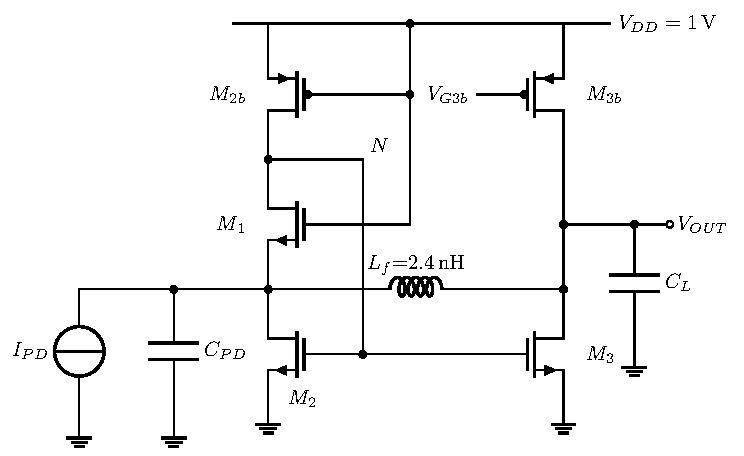
\includegraphics[height=4.2cm]{figures/schem_baseline}\hspace{1.2cm}
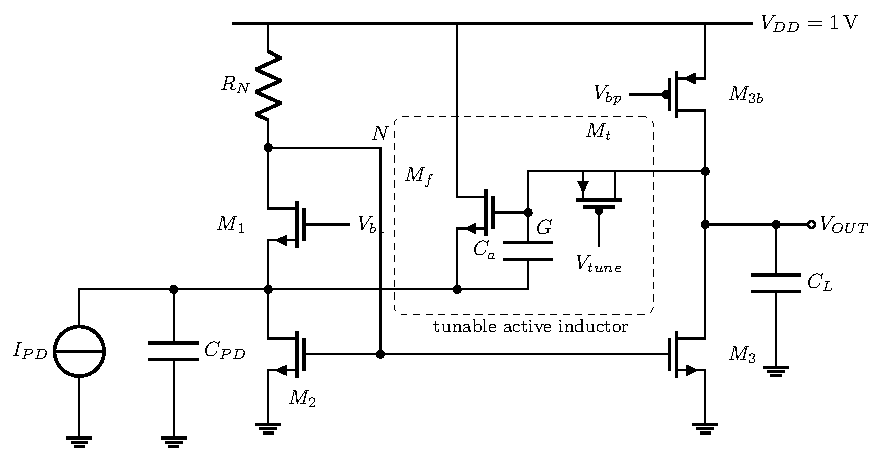
\includegraphics[height=4.2cm]{figures/schem_proposed}
\caption{(a) The 2020 baseline \cite{baseline} with a \SI{2.4}{nH} feedback spiral. (b) The proposed TIA. $M_f$ and $M_t$ with $C_a$ form the active inductor; $V_{b1}$ and the $M_{3b}$ gate come from the bias generator on the left.}
\label{fig:schem}
\end{figure*}

\section{The 2020 Baseline Re-examined}\label{sec:base}
\subsection{Operating point}
Fig.~\ref{fig:schem}(a) shows the baseline. $M_1$ is a common-gate device between the input and node $N$, $M_2$ and $M_3$ form the mirror, $M_{2b}$ and $M_{3b}$ are PMOS loads, and $L_f$ closes the loop. The predictive-model runs use ngspice~42 \cite{ngspice} with the 90\,nm Predictive Technology Model \cite{ptm} at \SI{1}{V} and \SI{35}{\celsius}. $C_{PD}=\SI{50}{fF}$ and $C_L=\SI{30}{fF}$ are assumed throughout.

The published schematic ties the gate of $M_{2b}$ to $V_{DD}$. $M_{2b}$ then has zero gate-source voltage and passes \BIOne\,nA, so $M_1$ has no bias current and sits in deep triode at \BGdsOne\,mS: a switch from node $N$ to the input. With $Z_f$ the feedback impedance and $g_o=g_{ds3}+g_{ds3b}$, nodal analysis gives
\begin{equation}
Z_T=\frac{1-g_{m3}Z_f}{(g_{m2}+g_{ds2})(1+g_oZ_f)+g_o+g_{m3}}.
\label{eq:ztb}
\end{equation}
At DC, $Z_f=0$ and $Z_T=1/(g_{m2}+g_{m3}+g_{ds2}+g_o)$, \BZtOhm\,$\Omega$ or \BZt\,dB$\Omega$ with $g_{m2}=g_{m3}=\BGmTwo$\,mS. As $\omega L_f$ grows the feedback falls away and the gain has to rise until the node capacitances take over. That rise is the \BPk\,dB peak at \BFpk\,GHz.

\subsection{Why the published curve is not reproduced}
The published response falls steadily from \SI{203}{\ohm} at \SI{1}{GHz} and has no resonance. The simulator, model and capacitances behind it are unknown, so each candidate explanation was tested by fitting $C_{PD}$ and $C_L$ to twelve points digitised from \cite{baseline} (Fig.~\ref{fig:diag}). The circuit as drawn misses by \DgRmsFitDrawn\,dB rms. Freeing both PMOS gate biases and a spiral loss of up to \SI{110}{\ohm} as well brings the error only to \DgRmsBestL\,dB, and the best fit still peaks near \SI{25}{GHz}. A screen of \DgNScreen\ bias points found no setting with less than \DgPkMin\,dB of peaking. If $L_f$ is allowed to shrink, the error falls to \DgRmsNoL\,dB below about \DgLfMax\,pH, with about \DgIdNoL\,\si{\micro A} in each mirror branch. The published curve therefore matches this topology with no effective inductor and about a fifth of the drawn bias current. It does not match the circuit as drawn.

\begin{figure*}[t]
\centering
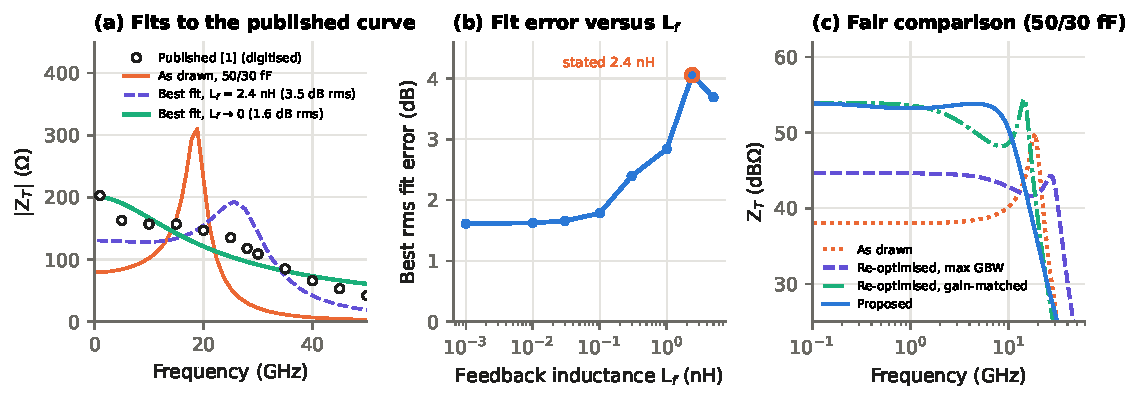
\includegraphics[width=0.9\textwidth]{figures/fig_baseline_diagnosis}
\caption{(a) Best fits to the published curve \cite{baseline} with the stated \SI{2.4}{nH} (biases, loss and capacitances free) and with $L_f$ free. (b) Best rms error against $L_f$. (c) The baseline as drawn, the two re-optimised baselines and the proposed TIA under the same conditions (PTM).}
\label{fig:diag}
\end{figure*}

\subsection{A fair reference}
A design compared against a circuit whose input device is in triode will look better than it is. The baseline topology was therefore re-optimised with the same search and constraints used for the proposed circuit: at most \SI{1}{dB} peaking, at most \SI{1.2}{mW}, $L_f$ from 0.2 to \SI{6}{nH} with up to \SI{60}{\ohm} of series loss, and the $M_{2b}$ gate given its own bias. Table~\ref{tab:reopt} gives two results. Optimised for gain-bandwidth product, the baseline reaches \RbGbw\,T$\Omega$Hz at \RbPow\,mW, slightly more than the proposed circuit and at about a quarter of its power. Its gain, though, is $1/(g_{m2}+g_{m3})$, so a high gain needs low transconductance. Held to the proposed circuit's gain it reaches only \RgBw\,GHz. This same-gain baseline is the reference used in the rest of the paper. In both cases the optimiser chose a lossy \SI{43}{\ohm} inductor, not the high-$Q$ spiral the original design assumed.

\begin{table}[t]
\caption{Baseline topology as drawn and re-optimised (PTM, $C_{PD}=\SI{50}{fF}$, $C_L=\SI{30}{fF}$, \SI{1}{V})}
\label{tab:reopt}
\centering\footnotesize\setlength{\tabcolsep}{3pt}
\begin{tabular}{|l|c|c|c|c|}
\hline
 & As drawn & Max GBW & Same gain & Proposed \\
\hline
Gain (dB$\Omega$) & \BZt & \RbZt & \RgZt & \PZt \\
BW (GHz) & resonant & \RbBw & \RgBw & \PBW \\
Peaking (dB) & \BPk & \RbPk & \RgPk & \PPk \\
Power (mW) & \BPow & \RbPow & \RgPow & \PPow \\
$i_n$ at \SI{5}{GHz} (pA/$\sqrt{\text{Hz}}$) & \BInFive & \RbInFive & \RgInFive & \PInFive \\
GBW (T$\Omega$Hz) & -- & \RbGbw & \RgGbw & \PGbw \\
Feedback & \SI{2.4}{nH} & \RbLf\,nH & \RgLf\,nH & active \\
\hline
\end{tabular}
\end{table}

\section{Proposed Circuit}\label{sec:prop}
\subsection{Topology and bias}
The proposed TIA (Fig.~\ref{fig:schem}b) changes three things. First, $M_{2b}$ becomes a \SI{5}{k\ohm} resistor $R_N$ and the gate of $M_1$ is driven from $V_{b1}$, so $M_1$ carries \IOne\,\si{\micro A} in saturation. $M_1$ and $M_2$ then form a flipped voltage follower \cite{fvf}, which lowers the input resistance in the way a regulated cascode does \cite{park}. The input settles at \Vin\,V instead of \BVin\,V. Second, $M_{3b}$ mirrors a \SI{50}{\micro A} reference, and $V_{b1}$ comes from a diode-connected replica of $M_1$ in series with $R_b$, so the bias no longer depends directly on the supply. Third, the spiral is replaced by the source follower $M_f$. Its source drives the input and its gate, node $G$, is fed from the output through the PMOS triode device $M_t$, whose gate is $V_{tune}$. $C_a$ sits between gate and source of $M_f$.

The level shift at the input is what makes room for $M_f$. It needs about \SI{0.4}{V} of gate-source drop, so the output sits at \Vout\,V and \SI{0.34}{V} is left across $M_{3b}$. $M_t$ carries no DC current, so changing $V_{tune}$ does not move the operating point. Table~\ref{tab:sizes} gives the sizes, found by a differential-evolution search that maximised bandwidth at no less than \SI{53}{dB\ohm}, no more than \SI{1}{dB} of peaking and \SI{1.2}{mW}, with every device in saturation. The circuit draws \ITot\,\si{\micro A}, \SI{97}{\micro A} of it in the bias generator.

\begin{table}[t]
\caption{Device sizes ($W/L$ in \si{\micro m}). $R_N=\SI{5}{k\ohm}$, $R_b=\SI{4.2}{k\ohm}$, $C_a=\SI{30}{fF}$, $I_{ref}=\SI{50}{\micro A}$}
\label{tab:sizes}
\centering\footnotesize
\begin{tabular}{|l|l|l|l|}
\hline
Device & $W/L$ & Device & $W/L$ \\
\hline
\tableinput table_sizes.tex
\hline
\end{tabular}
\end{table}

\subsection{The active inductor}
Seen from the input, with the output at AC ground, $M_f$ and its gate network present
\begin{equation}
Z_{AI}=\frac{1+sR_tC_g}{g_f+sC_g},\qquad L_{eq}=\frac{C_g}{g_f}\left(R_t-\frac{1}{g_f}\right),
\label{eq:zai}
\end{equation}
where $g_f=g_{mf}+g_{mbf}+g_{dsf}$, $C_g=C_a+C_{gsf}$ and $R_t$ is the channel resistance of $M_t$ \cite{yuan,sackingerla}. The element is inductive only when $R_t>1/g_f$. In simulation (Fig.~\ref{fig:ai}) the low-frequency resistance is \AIRs\,$\Omega$ and the impedance turns inductive near \SI{0.27}{V}. At \SI{1}{GHz} the equivalent inductance is \AILB, \AILC\ and \AILD\,nH at $V_{tune}=0.32$, 0.36 and \SI{0.40}{V}, with a peak $Q$ of only \AIQD. This is a very lossy inductor, and it is used as a movable zero, not as a resonator. It is also one-way: it injects a current set by the output voltage into the input, but draws no signal current from the output.

\begin{figure}[t]
\centering
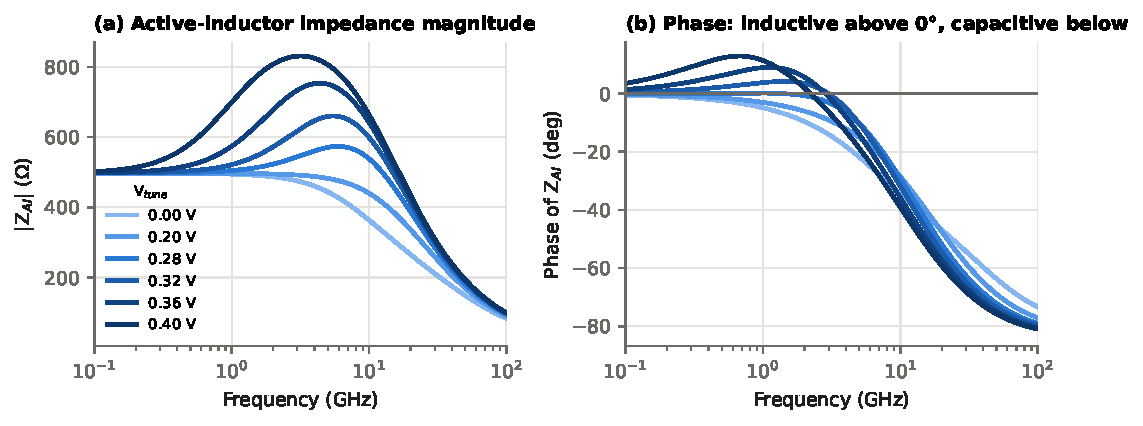
\includegraphics[width=\linewidth]{figures/fig_active_inductor}
\caption{Simulated impedance of the active inductor seen from the input, output at AC ground, for several $V_{tune}$ (PTM).}
\label{fig:ai}
\end{figure}

\subsection{Transimpedance}
Let $m=g_{m3}/g_{m2}$ be the mirror gain, $R_o$ the output resistance and $C_o$ the output capacitance. Closing the loop through $M_f$ gives
\begin{equation}
Z_T(s)\approx-\frac{mR_o(1+sR_tC_g)}{(1+sR_oC_o)(1+sR_tC_g)+m\,g_{mf}R_o}\,H_{in}(s),
\label{eq:zt}
\end{equation}
where $H_{in}$ is the second-order response of the input stage. At DC this is $-mR_o/(1+T_0)$ with loop gain $T_0=m\,g_{mf}R_o=\Tzero$, which gives \ZtApprox\,$\Omega$ against \PZtOhm\,$\Omega$ from SPICE. The gate network adds a zero at $1/(R_tC_g)$ and turns the output pole into a complex pair whose damping falls as $R_t$ rises. A small $R_t$ removes the feedback slowly and the response droops early; a larger $R_t$ flattens it; a still larger one makes it peak.

\section{Predictive-Model Results}\label{sec:ptm}
\subsection{Nominal point and noise}
At $V_{tune}=\VtNom$\,V the TIA gives \PZt\,dB$\Omega$, \PBW\,GHz with \PPk\,dB of peaking, and \PPow\,mW. The input-referred noise is \PInOne, \PInFive\ and \PInTen\,pA/$\sqrt{\text{Hz}}$ at 1, 5 and \SI{10}{GHz}, and \PIrms\,\si{\micro A} rms integrated over the bandwidth. At \SI{5}{GHz} (Fig.~\ref{fig:noise}) $M_1$ contributes \NsMOne\,\% of the output noise power, $M_2$ \NsMTwo\,\%, $M_3$ \NsMThree\,\%, and the feedback devices $M_f$ and $M_t$ together \SI{21}{\percent}. In the baseline as drawn the triode $M_1$ alone gives \NsBMOne\,\%, which is why it is noisier at \BInFive\,pA/$\sqrt{\text{Hz}}$ despite having fewer devices.

Against the same-gain baseline the proposed TIA has \BwRatioGain\ times the bandwidth, but about ten times the power and \PInFive\ against \RgInFive\,pA/$\sqrt{\text{Hz}}$ of noise.

\begin{figure}[t]
\centering
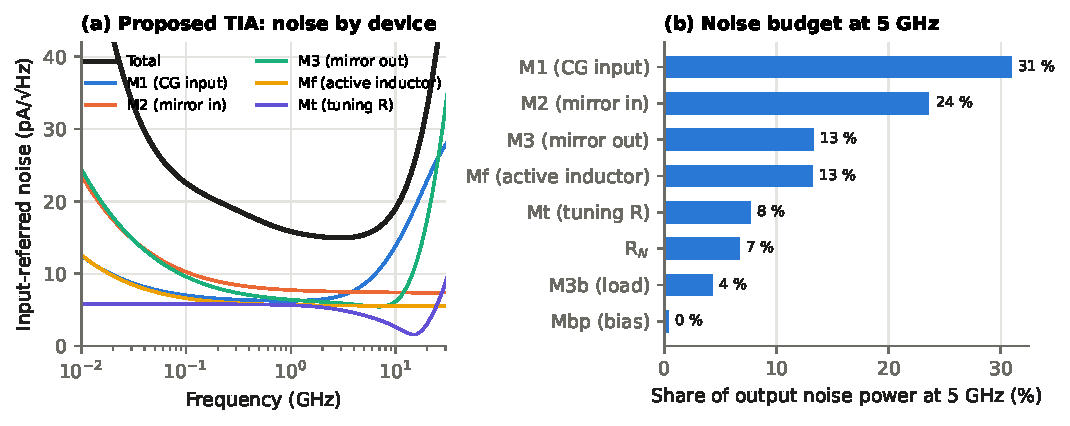
\includegraphics[width=\linewidth]{figures/fig_noise}
\caption{(a) Input-referred noise by device. (b) Share of output noise power at \SI{5}{GHz} (PTM).}
\label{fig:noise}
\end{figure}

\subsection{Tuning and stability}
Fig.~\ref{fig:tune} and Table~\ref{tab:tune} give the response against $V_{tune}$. As $R_t$ rises from \RtMin\ to \RtNom\,$\Omega$ between 0 and \SI{0.28}{V}, the bandwidth moves from \TuneMin\ to \PBW\,GHz and the gain and peaking do not change. Above \SI{0.30}{V} the bandwidth stops rising and the peaking grows, to \SI{3.86}{dB} at \SI{0.40}{V}. The lower settings also cut the integrated noise, to \IrmsMin\,\si{\micro A} at \SI{0}{V}, which suits a lower data rate.

\begin{figure}[t]
\centering
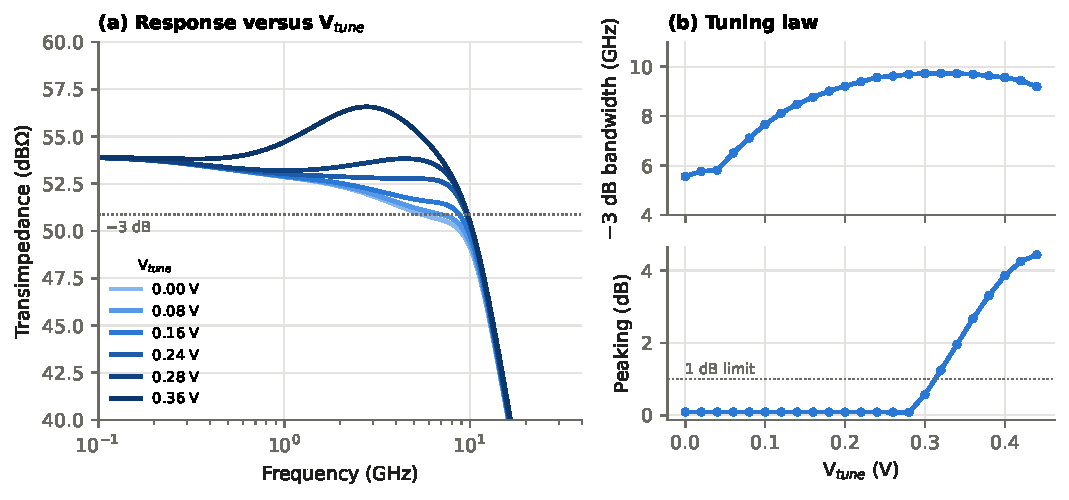
\includegraphics[width=\linewidth]{figures/fig_vtune_tuning}
\caption{(a) Transimpedance and (b) bandwidth and peaking against $V_{tune}$ (PTM).}
\label{fig:tune}
\end{figure}

\begin{table}[t]
\caption{Tuning law (PTM, nominal, \SI{1}{V}, \SI{35}{\celsius})}
\label{tab:tune}
\centering\footnotesize\setlength{\tabcolsep}{3pt}
\begin{tabular}{|c|c|c|c|c|c|}
\hline
$V_{tune}$ & $R_t$ & BW & Peak & $i_{n,rms}$ & $i_n$ at \SI{5}{GHz} \\
(V) & ($\Omega$) & (GHz) & (dB) & (\si{\micro A}) & (pA/$\sqrt{\text{Hz}}$) \\
\hline
\tableinput table_tune.tex
\hline
\end{tabular}
\end{table}

Loop gains were measured with Middlebrook's double injection \cite{middlebrook}. The global loop has \LoopTzero\,dB of DC gain, crosses unity between \LoopFuMin\ and \LoopFuMax\,GHz and keeps at least \LoopPMg\si{\degree} of phase margin over the tuning range. The local flipped-voltage-follower loop is the tighter one: \LoopPMl\si{\degree} at \SI{50}{fF} of photodiode capacitance, falling to \LoopPMlCpd\si{\degree} at \SI{200}{fF}.

\subsection{Corners and mismatch}
The PTM card has no foundry corners, so they were emulated with $\pm\SI{30}{mV}$ threshold and $\pm\SI{5}{\percent}$ mobility shifts for each device type, $\pm\SI{15}{\percent}$ on resistors and $\pm\SI{10}{\percent}$ on $C_a$, together with 0.9 and \SI{1.1}{V} supplies and $-40$ and \SI{85}{\celsius}. Over fifteen such conditions with $V_{tune}$ fixed, the bandwidth spans \PvtBwMin\ to \PvtBwMax\,GHz and the peaking reaches \PvtPkMax\,dB, in the FS case. Choosing $V_{tune}$ per condition on a \SI{20}{mV} grid holds the peaking to \PvtPkTMax\,dB (Fig.~\ref{fig:pvt}). Trimming cannot recover bandwidth the input stage loses when slow and hot: SS at \SI{0.9}{V} and \SI{85}{\celsius} stays at \PvtBwTMin\,GHz.

\begin{figure}[t]
\centering
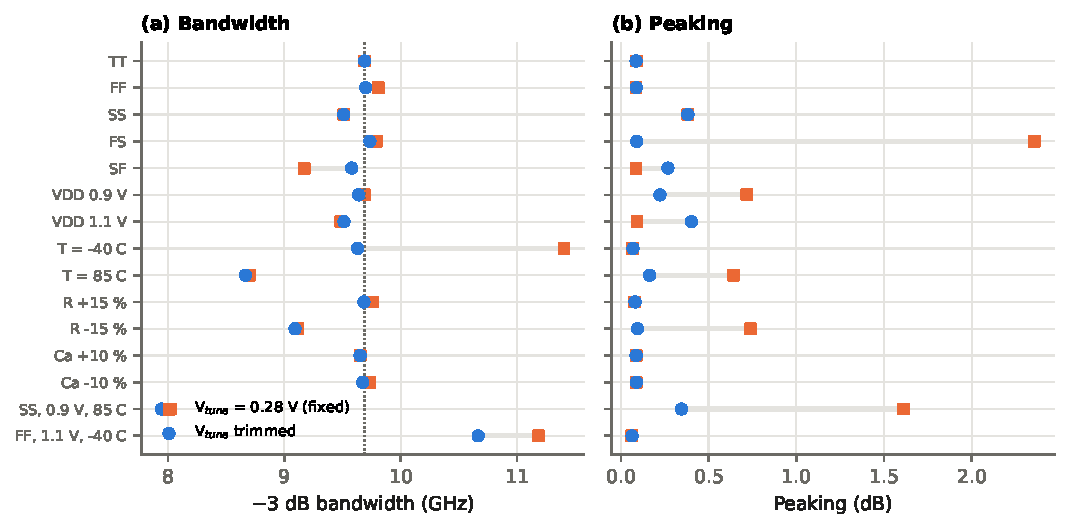
\includegraphics[width=\linewidth]{figures/fig_pvt}
\caption{Bandwidth and peaking over fifteen emulated corner, supply and temperature conditions with fixed and trimmed $V_{tune}$ (PTM). The dotted line is the nominal bandwidth.}
\label{fig:pvt}
\end{figure}

A \McN-sample Monte Carlo run combined global spread with Pelgrom mismatch \cite{pelgrom} at $A_{VT}=\SI{3.5}{mV.\micro m}$ and $A_\beta=\SI{1}{\percent.\micro m}$, both assumed. With $V_{tune}$ fixed the bandwidth is $\McBwMean\pm\McBwStd$\,GHz and \McPkYieldFixed\,\% of samples stay under \SI{1}{dB} of peaking. With the same trimming rule every sample does, the worst being \McPkTMax\,dB (Fig.~\ref{fig:mc}).

\begin{figure}[t]
\centering
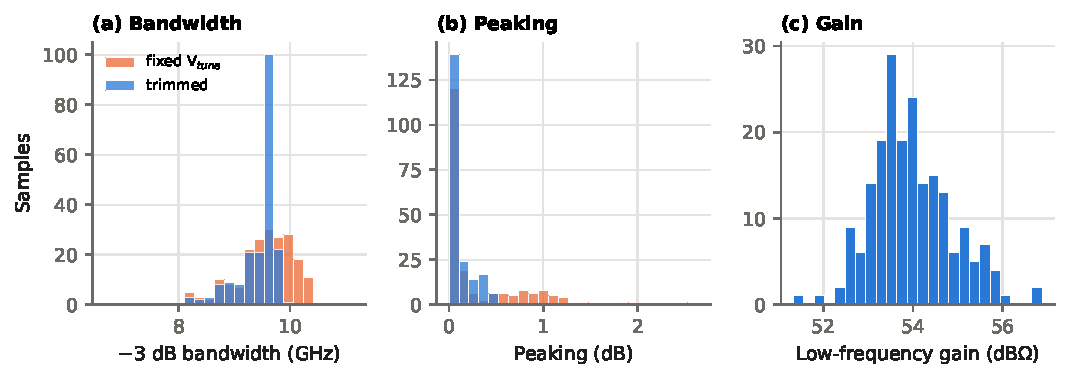
\includegraphics[width=\linewidth]{figures/fig_monte_carlo}
\caption{Monte Carlo distributions (\McN\ samples, PTM) with fixed and trimmed $V_{tune}$.}
\label{fig:mc}
\end{figure}

\subsection{Eye diagrams}
For a $2^7-1$ pseudo-random input of \SI{100}{\micro A} peak to peak, the test current of \cite{baseline}, the proposed TIA gives a \EyePTenAmp\,mV swing at \SI{10}{Gb/s} with a vertical opening of \EyePTenPct\,\% and a horizontal opening of \EyePTenW\,\% of the unit interval (Fig.~\ref{fig:eye}). At \SI{12.5}{Gb/s} it keeps \EyePTwW\,\% horizontally, while ringing at the baseline's resonance closes its eye to \EyeBTwW\,\%.

\begin{figure}[t]
\centering
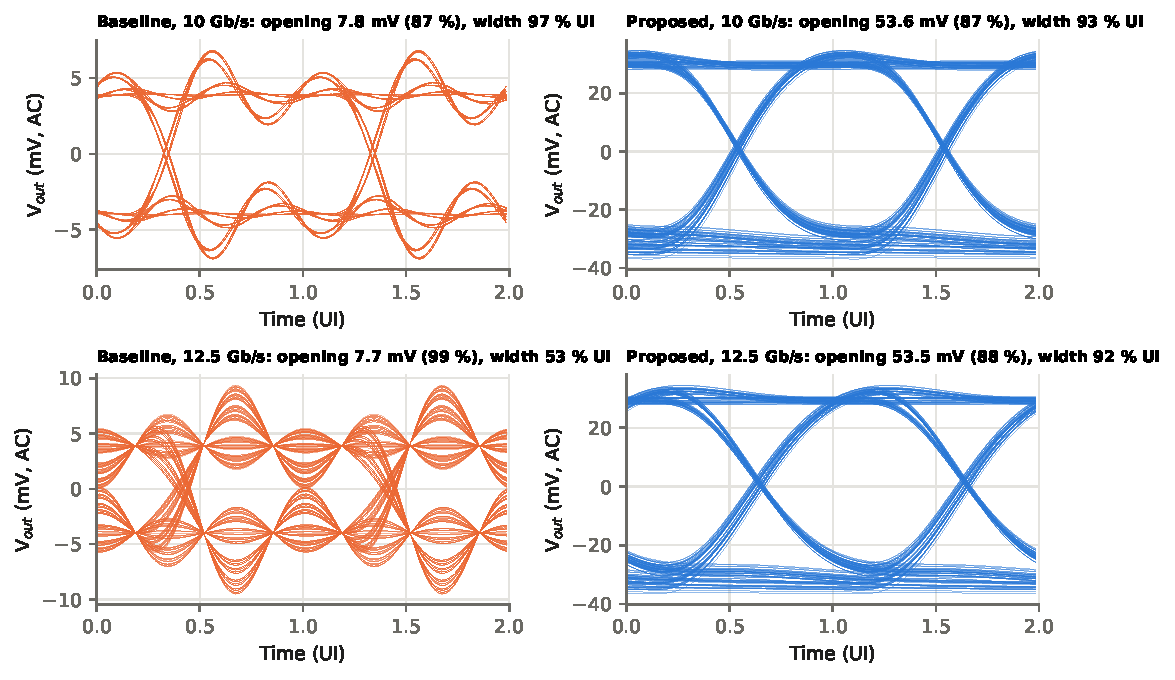
\includegraphics[width=\linewidth]{figures/fig_eye_diagrams}
\caption{Eye diagrams for a \SI{100}{\micro A} peak-to-peak PRBS-7 input, no noise (PTM).}
\label{fig:eye}
\end{figure}

\subsection{Load and photodiode capacitance}
Fig.~\ref{fig:load}(a) compares the active-inductor network with plain follower feedback, where the gate of $M_f$ is tied to the output and $C_a$ is removed. At the nominal \SI{30}{fF} load the plain follower is faster, \LdResLight\ against \LdAiLight\,GHz, because the input stage sets the bandwidth and the gate network only adds capacitance. As the load grows the output pole takes over and the inductive zero starts to pay: re-tuned, the active inductor gives \LdRatioMid\ times the plain follower's bandwidth at \SI{150}{fF} and \LdRatioHeavy\ times at \SI{250}{fF}. With a larger photodiode the peaking grows, and lowering $V_{tune}$ keeps it under \SI{1}{dB} up to \SI{200}{fF} at about \SI{7.4}{GHz} (Fig.~\ref{fig:load}b).

\begin{figure}[t]
\centering
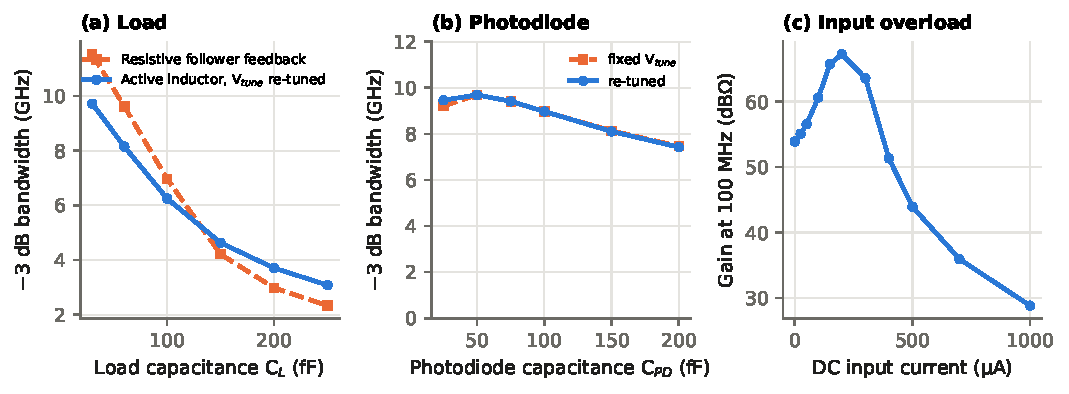
\includegraphics[width=\linewidth]{figures/fig_load_pd_overload}
\caption{(a) Bandwidth against load for plain follower feedback and the re-tuned active inductor. (b) Bandwidth against photodiode capacitance. (c) Gain at \SI{100}{MHz} against DC input current (PTM).}
\label{fig:load}
\end{figure}

\subsection{Input overload and DC cancellation}
Average photocurrent flowing into the input is taken from $M_f$, which carries \IF\,\si{\micro A}. The gain moves by more than \SI{1}{dB} above \PrLimit\,\si{\micro A}, and by \SI{100}{\micro A} $M_f$ is starved (Fig.~\ref{fig:load}c) and the bandwidth has fallen to \PrBwHundred\,GHz. The loop in Fig.~\ref{fig:dccs} protects the follower current directly. Because $M_t$ carries no DC current, $V_{OUT}-V_{IN}$ is the gate-source voltage of $M_f$. A half-width replica $M_r$ biased at $I_{th}/2$ gives $V_R=V_{OUT}-V_{GS}(I_{th})$, and a PMOS-input OTA integrates $V_R-V_{IN}$ on \SI{2}{pF} and drives $M_{dc}$ to sink the excess photocurrent. The threshold sits just above the dark follower current, so the loop is always engaged; a threshold below it failed in Monte Carlo.

With the loop (Fig.~\ref{fig:dcc}) the bandwidth stays within \SI{10}{\percent} and the gain within \SI{1}{dB} of their dark values up to \DcLimit\,\si{\micro A}. It costs \DcPowAdd\,\si{\micro W}, \SI{0.5}{dB} of gain and \DcNoisePct\,\% more noise at \SI{5}{GHz}, and it has at least \DcPmMin\si{\degree} of phase margin. Its low-frequency corner rises to \DcFloMax\,MHz at \SI{500}{\micro A}, which limits long runs of identical bits.

\begin{figure}[t]
\centering
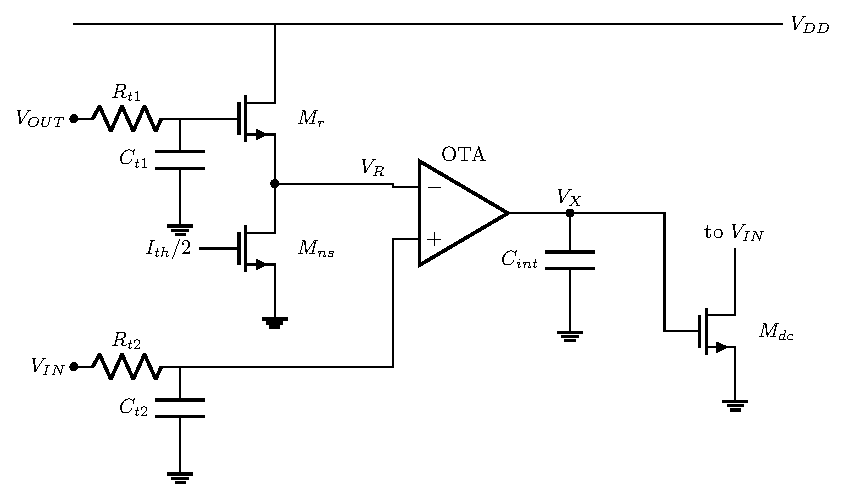
\includegraphics[width=0.9\linewidth]{figures/schem_dcc}
\caption{DC-cancellation loop. $V_{OUT}$ and $V_{IN}$ are the nodes of Fig.~\ref{fig:schem}(b).}
\label{fig:dccs}
\end{figure}

\begin{figure*}[t]
\centering
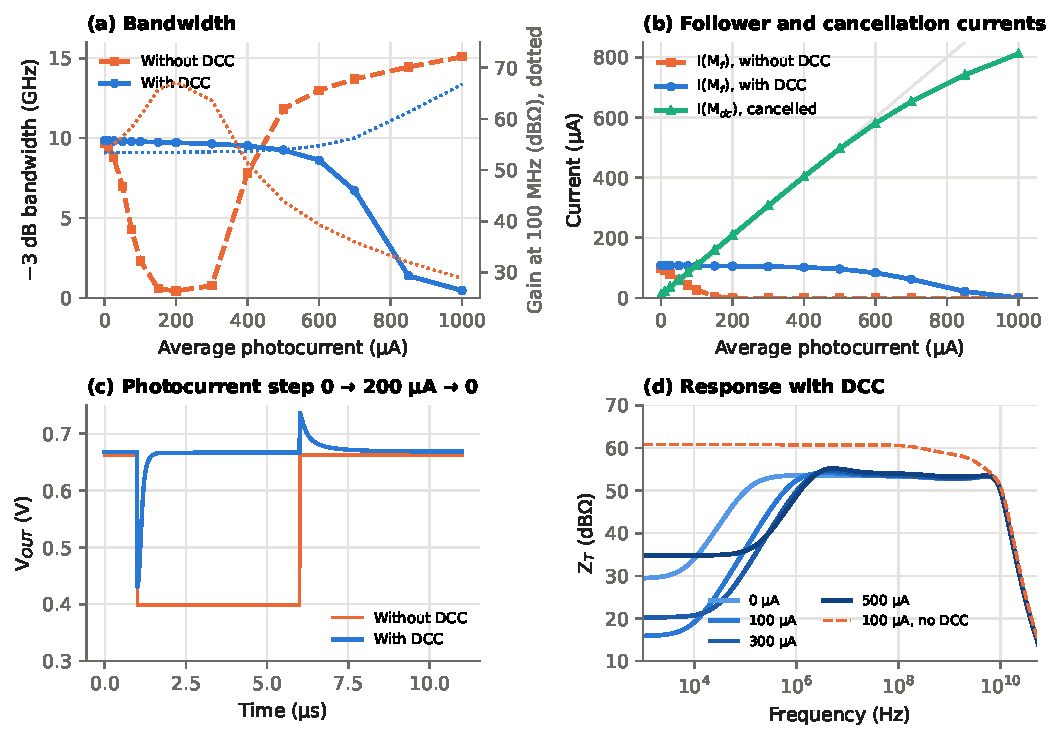
\includegraphics[width=0.78\textwidth]{figures/fig_dcc}
\caption{DC-cancellation loop (PTM). (a) Bandwidth (solid) and gain at \SI{100}{MHz} (dotted) against average photocurrent. (b) Follower and cancellation currents. (c) Output for a photocurrent step. (d) Transimpedance at several average currents.}
\label{fig:dcc}
\end{figure*}

\section{GPDK090 Cross-Check}\label{sec:gpdk}
The predictive model is not a foundry model, so the three circuits that carry the argument were rebuilt as Virtuoso schematics and simulated in Spectre with the GPDK090 v4.6 models (\texttt{nmos1v}, \texttt{pmos1v}). The kit's minimum length is \SI{100}{nm}, so every device uses $L\geq\SI{100}{nm}$ with the widths of Table~\ref{tab:sizes}, and the numbers are not expected to match the PTM ones exactly. $V_{tune}$ is \SI{0.24}{V}. The same-gain baseline is the 2020 topology re-biased to the proposed circuit's gain, with a \SI{43}{\ohm} feedback series resistor and fixed gate-bias sources. Gain is read at \SI{100}{MHz}.

\begin{table}[t]
\caption{GPDK090 nominal point (NN, \SI{35}{\celsius}, \SI{1}{V})}
\label{tab:gnom}
\centering\footnotesize\setlength{\tabcolsep}{3pt}
\begin{tabular}{|l|c|c|c|c|c|}
\hline
Circuit & Gain & Peak & BW & $I_{DD}$ & $i_n$ at \SI{5}{GHz} \\
 & (dB$\Omega$) & (dB) & (GHz) & (mA) & (pA/$\sqrt{\text{Hz}}$) \\
\hline
\tableinput table_gpdk_nom_c.tex
\hline
\end{tabular}
\end{table}

\begin{table}[t]
\caption{GPDK090 range over NN, SS, FF, FS and SF at $-40$, 35 and \SI{125}{\celsius}, $V_{tune}$ fixed}
\label{tab:gcorn}
\centering\footnotesize\setlength{\tabcolsep}{3pt}
\begin{tabular}{|l|c|c|c|c|}
\hline
Circuit & Gain (dB$\Omega$) & BW (GHz) & Peak (dB) & $I_{DD}$ (mA) \\
\hline
\tableinput table_gpdk_corner_c.tex
\hline
\end{tabular}
\end{table}

Table~\ref{tab:gnom} gives the nominal results. The 2020 baseline as drawn gives \SI{40.5}{dB\ohm} with \SI{8.9}{dB} of peaking, so the foundry models agree that the published flat response does not come from this circuit. The same-gain baseline gives \SI{3.3}{GHz} at \SI{0.07}{mA}, close to its PTM figures. The proposed circuit gives \SI{53.8}{dB\ohm} and \SI{7.8}{GHz} at \SI{0.97}{mA}. That is 2.3 times the bandwidth of the same-gain baseline, for fourteen times the current and 1.8 times the noise density. Integrated from \SI{10}{MHz} to \SI{10}{GHz}, the input noise is \SI{1.77}{\micro A} for the proposed circuit and \SI{0.87}{\micro A} for the same-gain baseline.

Over fifteen corner and temperature points (Table~\ref{tab:gcorn}) the proposed circuit's gain stays within \SI{3.2}{dB} and its current within \SI{0.16}{mA}. The same-gain baseline's gain moves by \SI{11.1}{dB} and its bandwidth from 1.6 to \SI{16.8}{GHz}, partly because its gate biases are fixed voltages rather than tracking a reference. With $V_{tune}$ fixed, the proposed circuit peaks by \SI{4.2}{dB} in FS at \SI{-40}{\celsius}. Per-corner trimming, which removed such peaking with the predictive model, has not yet been run with the foundry models.

The tuning range is where the two models disagree most. Sweeping $V_{tune}$ from 0 to \SI{0.30}{V} moves the GPDK090 bandwidth from 5.70 to \SI{7.88}{GHz}, a ratio of 1.38 against \TuneRatio\ with PTM. The gain stays at \SI{53.8}{dB\ohm} and the peaking stays below \SI{1}{dB} up to \SI{0.28}{V}, reaching \SI{3.5}{dB} at \SI{0.40}{V}.

\section{Comparison and Limitations}
Table~\ref{tab:comp} places the results beside related work. Other designs are listed as their authors report them. The proposed circuit is not more efficient than a well-biased baseline. What it offers is bandwidth at high gain, feedback without a spiral, and a control voltage for bandwidth and corner peaking.

\begin{table}[t]
\caption{Comparison (sim.: simulated, meas.: measured)}
\label{tab:comp}
\centering\footnotesize\setlength{\tabcolsep}{2.2pt}
\begin{tabular}{|l|c|c|c|c|c|}
\hline
Work & Node & Gain & BW & Power & Tun- \\
 & & (dB$\Omega$) & (GHz) & (mW) & able \\
\hline
\cite{baseline} published & 90\,nm & 43.9 & 5--15 & n/r & no \\
\cite{baseline} as drawn, PTM & 90\,nm & \BZt & resonant & \BPow & no \\
Same-gain base., GPDK & 90\,nm & 55.4 & 3.3 & 0.07 & no \\
\cite{zohoori} sim. & 90\,nm & 40.5 & 7 & 1.4 & no \\
\cite{issa} sim. & 45\,nm & 68.2 & 2.5 & 0.56 & no \\
\cite{hwang} meas. & 180\,nm & 52 & 3.9--7.6 & 34 & yes \\
\cite{chien} meas. & 180\,nm & 47.8 & 6.2--10.5 & 33.3 & yes \\
This work, PTM & 90\,nm & \PZt & \TuneMin--\TuneMax & \PPow & yes \\
This work, GPDK & 90\,nm & 53.8 & 5.7--7.9 & 0.97 & yes \\
\hline
\end{tabular}
\end{table}

All results are schematic-level. Layout parasitics at the input and at node $N$ will lower the bandwidth. Mismatch, eye diagrams, loop gains and the DC-cancellation loop were simulated only with the predictive model, and its corners are emulated. The photodiode is modelled as a current source and a capacitor, without bond-wire inductance or ESD protection, and the reference current is ideal. The diagnosis of the 2020 circuit rests on digitised points and assumed capacitances.

\section{Conclusion}
The 2020 current-mirror TIA does not give its published response as drawn with a \SI{2.4}{nH} inductor, with either the predictive or the foundry models. Replacing the spiral with a voltage-tuned source-follower active inductor, and biasing the input as a flipped voltage follower, gives \SI{53.8}{dB\ohm} and \SI{7.8}{GHz} at \SI{0.97}{mA} with GPDK090, against \SI{3.3}{GHz} at \SI{0.07}{mA} for a baseline at the same gain. One voltage sets the bandwidth, over 1.75:1 with the predictive model and 1.38:1 with the foundry models. The next steps are per-corner trimming and Monte Carlo with the foundry kit, followed by layout.

\begin{thebibliography}{00}
\bibitem{razavi} B. Razavi, \emph{Design of Integrated Circuits for Optical Communications}, 2nd ed. Hoboken, NJ, USA: Wiley, 2012.
\bibitem{sackinger} E. S\"ackinger, \emph{Analysis and Design of Transimpedance Amplifiers for Optical Receivers}. Hoboken, NJ, USA: Wiley, 2017.
\bibitem{zohoori} S. Zohoori, M. Dolatshahi, M. Pourahmadi, and M. Hajisafari, ``A CMOS low-power current-mirror-based transimpedance amplifier for 10 Gbps optical communications,'' \emph{Microelectron. J.}, vol. 80, pp. 18--27, 2018.
\bibitem{hassan} M. Hassan and H. Zimmermann, ``A 10Gb/s inductor less push pull current mirror transimpedance amplifier,'' in \emph{Proc. IEEE Int. Conf. Electron., Circuits Syst. (ICECS)}, Seville, Spain, 2012.
\bibitem{issa} M. S. H. Alsheikhjader and A. A. Issa, ``A simulated 45 nm MOSFET channel process in transimpedance amplifier design for optoelectronics applications,'' \emph{Jordan J. Phys.}, vol. 17, no. 2, pp. 165--178, 2024.
\bibitem{alyas} M. M. Alyas and M. S. H. Alsheikhjader, ``A low-power 45 nm CMOS transimpedance amplifier with active inductor feedback for fiber-optic applications,'' \emph{Jordan J. Phys.}, vol. 19, no. 2, pp. 131--143, 2026.
\bibitem{shaaban} Shaaban \emph{et al.}, ``Design of a novel CMOS transimpedance amplifier based on a current mirror,'' \emph{Int. J. Circuit Theory Appl.}, 2025, doi: 10.1002/cta.4353.
\bibitem{mohanbw} S. S. Mohan, M. del M. Hershenson, S. P. Boyd, and T. H. Lee, ``Bandwidth extension in CMOS with optimized on-chip inductors,'' \emph{IEEE J. Solid-State Circuits}, vol. 35, no. 3, pp. 346--355, Mar. 2000.
\bibitem{yuan} F. Yuan, \emph{CMOS Active Inductors and Transformers: Principle, Implementation, and Applications}. New York, NY, USA: Springer, 2008.
\bibitem{razaviai} B. Razavi, ``The active inductor [A circuit for all seasons],'' \emph{IEEE Solid-State Circuits Mag.}, vol. 12, no. 2, pp. 7--11, 2020.
\bibitem{baseline} M. S. H. Alsheikhjader, ``Low noise with wide band transimpedance amplifier for nonlinear fiber optical applications,'' \emph{Rafidain J. Sci.}, vol. 29, no. 1, pp. 71--78, 2020, doi: 10.33899/rjs.2020.164476.
\bibitem{alberwari} R. A. Al-Berwari and M. S. H. Alsheikhjader, ``An active inductor based transimpedance amplifier with two local feedbacks as a fiber optic application,'' \emph{Rafidain J. Sci.}, vol. 32, no. 2, pp. 38--52, 2023, doi: 10.33899/rjs.2023.178574.
\bibitem{hwang} H.-Y. Hwang, J.-C. Chien, T.-Y. Chen, and L.-H. Lu, ``A CMOS tunable transimpedance amplifier,'' \emph{IEEE Microw. Wireless Compon. Lett.}, vol. 16, no. 12, pp. 693--695, Dec. 2006.
\bibitem{chien} C.-K. Chien, H.-H. Hsieh, H.-S. Chen, and L.-H. Lu, ``A transimpedance amplifier with a tunable bandwidth in 0.18-$\mu$m CMOS,'' \emph{IEEE Trans. Microw. Theory Techn.}, vol. 58, no. 3, pp. 498--505, Mar. 2010.
\bibitem{ngspice} H. Vogt \emph{et al.}, \emph{Ngspice User's Manual}, version 42, 2023.
\bibitem{ptm} W. Zhao and Y. Cao, ``New generation of predictive technology model for sub-45 nm early design exploration,'' \emph{IEEE Trans. Electron Devices}, vol. 53, no. 11, pp. 2816--2823, Nov. 2006.
\bibitem{fvf} R. G. Carvajal \emph{et al.}, ``The flipped voltage follower: A useful cell for low-voltage low-power circuit design,'' \emph{IEEE Trans. Circuits Syst. I, Reg. Papers}, vol. 52, no. 7, pp. 1276--1291, Jul. 2005.
\bibitem{park} S. M. Park and H.-J. Yoo, ``1.25-Gb/s regulated cascode CMOS transimpedance amplifier for Gigabit Ethernet applications,'' \emph{IEEE J. Solid-State Circuits}, vol. 39, no. 1, pp. 112--121, Jan. 2004.
\bibitem{sackingerla} E. S\"ackinger and W. C. Fischer, ``A 3-GHz 32-dB CMOS limiting amplifier for SONET OC-48 receivers,'' \emph{IEEE J. Solid-State Circuits}, vol. 35, no. 12, pp. 1884--1888, Dec. 2000.
\bibitem{middlebrook} R. D. Middlebrook, ``Measurement of loop gain in feedback systems,'' \emph{Int. J. Electron.}, vol. 38, no. 4, pp. 485--512, 1975.
\bibitem{pelgrom} M. J. M. Pelgrom, A. C. J. Duinmaijer, and A. P. G. Welbers, ``Matching properties of MOS transistors,'' \emph{IEEE J. Solid-State Circuits}, vol. 24, no. 5, pp. 1433--1439, Oct. 1989.
\end{thebibliography}
\end{document}
